\documentclass[12pt,letterpaper]{article}
\usepackage{graphicx,textcomp}
\usepackage{natbib}
\usepackage{setspace}
\usepackage{fullpage}
\usepackage{color}
\usepackage[reqno]{amsmath}
\usepackage{amsthm}
\usepackage{fancyvrb}
\usepackage{amssymb,enumerate}
\usepackage[all]{xy}
\usepackage{endnotes}
\usepackage{lscape}
\newtheorem{com}{Comment}
\usepackage{float}
\usepackage{hyperref}
\newtheorem{lem} {Lemma}
\newtheorem{prop}{Proposition}
\newtheorem{thm}{Theorem}
\newtheorem{defn}{Definition}
\newtheorem{cor}{Corollary}
\newtheorem{obs}{Observation}
\usepackage[compact]{titlesec}
\usepackage{dcolumn}
\usepackage{tikz}
\usetikzlibrary{arrows}
\usepackage{multirow}
\usepackage{xcolor}
\newcolumntype{.}{D{.}{.}{-1}}
\newcolumntype{d}[1]{D{.}{.}{#1}}
\definecolor{light-gray}{gray}{0.65}
\usepackage{url}
\usepackage{listings}
\usepackage{color}

\definecolor{codegreen}{rgb}{0,0.6,0}
\definecolor{codegray}{rgb}{0.5,0.5,0.5}
\definecolor{codepurple}{rgb}{0.58,0,0.82}
\definecolor{backcolour}{rgb}{0.95,0.95,0.92}

\lstdefinestyle{mystyle}{
	backgroundcolor=\color{backcolour},   
	commentstyle=\color{codegreen},
	keywordstyle=\color{magenta},
	numberstyle=\tiny\color{codegray},
	stringstyle=\color{codepurple},
	basicstyle=\footnotesize,
	breakatwhitespace=false,         
	breaklines=true,                 
	captionpos=b,                    
	keepspaces=true,                 
	numbers=left,                    
	numbersep=5pt,                  
	showspaces=false,                
	showstringspaces=false,
	showtabs=false,                  
	tabsize=2
}
\lstset{style=mystyle}
\newcommand{\Sref}[1]{Section~\ref{#1}}
\newtheorem{hyp}{Hypothesis}

\title{Problem Set 3}
\date{Due: March 26, 2023}
\author{Daniel Murray (13303981)}


\begin{document}
	\maketitle
	\section*{Instructions}
	\begin{itemize}
	\item Please show your work! You may lose points by simply writing in the answer. If the problem requires you to execute commands in \texttt{R}, please include the code you used to get your answers. Please also include the \texttt{.R} file that contains your code. If you are not sure if work needs to be shown for a particular problem, please ask.
\item Your homework should be submitted electronically on GitHub in \texttt{.pdf} form.
\item This problem set is due before 23:59 on Sunday March 26, 2023. No late assignments will be accepted.
	\end{itemize}

	\vspace{.25cm}
\section*{Question 1}
\vspace{.25cm}
\noindent We are interested in how governments' management of public resources impacts economic prosperity. Our data come from \href{https://www.researchgate.net/profile/Adam_Przeworski/publication/240357392_Classifying_Political_Regimes/links/0deec532194849aefa000000/Classifying-Political-Regimes.pdf}{Alvarez, Cheibub, Limongi, and Przeworski (1996)} and is labelled \texttt{gdpChange.csv} on GitHub. The dataset covers 135 countries observed between 1950 or the year of independence or the first year forwhich data on economic growth are available ("entry year"), and 1990 or the last year for which data on economic growth are available ("exit year"). The unit of analysis is a particular country during a particular year, for a total $>$ 3,500 observations. 

\begin{itemize}
	\item
	Response variable: 
	\begin{itemize}
		\item \texttt{GDPWdiff}: Difference in GDP between year $t$ and $t-1$. Possible categories include: "positive", "negative", or "no change"
	\end{itemize}
	\item
	Explanatory variables: 
	\begin{itemize}
		\item
		\texttt{REG}: 1=Democracy; 0=Non-Democracy
		\item
		\texttt{OIL}: 1=if the average ratio of fuel exports to total exports in 1984-86 exceeded 50\%; 0= otherwise
	\end{itemize}
	
\end{itemize}
\newpage
\noindent Please answer the following questions:

\begin{enumerate}
	\item Construct and interpret an unordered multinomial logit with \texttt{GDPWdiff} as the output and "no change" as the reference category, including the estimated cutoff points and coefficients.
	
	\vspace{.5cm}
	\textbf{Answer:}\\
	
	The data was read in, inspected and wrangled to change the explanatory variables \texttt{REG} and \texttt{OIL} to factors and the outcome variable \texttt{GDPWdiff} to an unordered factor with three levels: "negative", "no change", and "positive". The category "no change" was then set as the reference category. See code used below:
	
	\vspace{.5cm}
	\lstinputlisting[language=R, firstline=39, lastline=58]{PS3_DanielMurray.R}  
	\vspace{.5cm} 
	
	Following this, a multinomial logit regression was run using the below code:
	
	\vspace{.5cm}
	\lstinputlisting[language=R, firstline=60, lastline=63]{PS3_DanielMurray.R}  
	\vspace{.5cm} 
	
	This produced the output in Table 1 below. The output shows that being a democracy leads to a an increase of 1.379 in the log odds of moving from "no change" to "negative", on average, holding the other variables constant. Having fuel exports make up over 50\% of total exports on average during 1984-1986 increases the log odds of moving from "no change to "negative" by 4.787 on average, holding other variables constant. For a non-democracy with less that 50\% of average total exports coming from fuel during 1984-1986, the log odds of moving from "no change" to "negative" is 3.805 on average.
	
	Similarly, being a democracy leads to a an increase of 1.769 in the log odds of moving from "no change" to "positive", on average, holding the other variables constant. Having fuel exports make up over 50\% of total exports on average during 1984-1986 increases the log odds of moving from "no change to "positive" by 4.576 on average, holding other variables constant. For a non-democracy with less that 50\% of average total exports coming from fuel during 1984-1986, the log odds of moving from "no change" to "positive" is 4.534 on average.
	
	% Table created by stargazer v.5.2.3 by Marek Hlavac, Social Policy Institute. E-mail: marek.hlavac at gmail.com
	% Date and time: Thu, Mar 23, 2023 - 18:02:44
	\begin{table}[H] \centering 
		\caption{} 
		\label{} 
		\begin{tabular}{@{\extracolsep{5pt}}lcc} 
			\\[-1.8ex]\hline 
			\hline \\[-1.8ex] 
			& \multicolumn{2}{c}{\textit{Dependent variable:}} \\ 
			\cline{2-3} 
			\\[-1.8ex] & negative & positive \\ 
			\\[-1.8ex] & (1) & (2)\\ 
			\hline \\[-1.8ex] 
			REG1 & 1.379$^{*}$ & 1.769$^{**}$ \\ 
			& (0.769) & (0.767) \\ 
			& & \\ 
			OIL1 & 4.784 & 4.576 \\ 
			& (6.885) & (6.885) \\ 
			& & \\ 
			Constant & 3.805$^{***}$ & 4.534$^{***}$ \\ 
			& (0.271) & (0.269) \\ 
			& & \\ 
			\hline \\[-1.8ex] 
			Akaike Inf. Crit. & 4,690.770 & 4,690.770 \\ 
			\hline 
			\hline \\[-1.8ex] 
			\textit{Note:}  & \multicolumn{2}{r}{$^{*}$p$<$0.1; $^{**}$p$<$0.05; $^{***}$p$<$0.01} \\ 
		\end{tabular} 
	\end{table} 
	
	\item Construct and interpret an ordered multinomial logit with \texttt{GDPWdiff} as the outcome variable, including the estimated cutoff points and coefficients.
	
	\vspace{.5cm}
	\textbf{Answer:}\\
	
	To run an ordered multinomial logit regression, the outcome variable was first changed to an ordered factor with levels set in the following order: "negative", "no change", "positive". The below code was used:
	
	\vspace{.5cm}
	\lstinputlisting[language=R, firstline=65, lastline=69]{PS3_DanielMurray.R}  
	\vspace{.5cm} 
	
	Next, the model was run using the below code:
	
	\vspace{.5cm}
	\lstinputlisting[language=R, firstline=71, lastline=73]{PS3_DanielMurray.R}  
	\vspace{.5cm} 

	This produced the output in Figure 1 below. The output shows that being a democracy is associated with a 0.3985 increase in the log odds of moving from "negative" to "no change", or from "no change" to positive", holding the other variable \texttt{OIL} constant. Having fuel exports make up over 50\% of total exports on average during 1984-1986 is associated with a 0.1987 decrease in the log odds of moving from "negative" to "no change", or from "no change" to positive", holding the other variable \texttt{REG} constant. The cutoff where our estimated outcome changes from "negative" to "no change" is where the value of log odds is equal to -0.7312. The cutoff where our estimated outcome changes from "no change" to "positive" is where the value of log odds is equal to -0.7105.
	
		\begin{figure}[H]\centering
		\caption{\footnotesize Output of ordered multinomial regression model}
		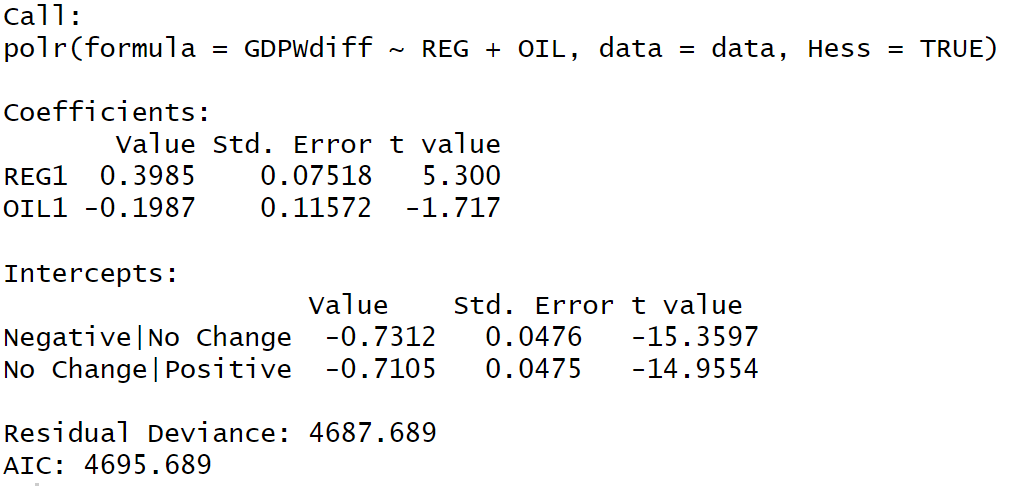
\includegraphics[width=.75\textwidth]{orderedMultinomOutput.png}
		\end{figure} 
	
\end{enumerate}

\section*{Question 2} 
\vspace{.25cm}

\noindent Consider the data set \texttt{MexicoMuniData.csv}, which includes municipal-level information from Mexico. The outcome of interest is the number of times the winning PAN presidential candidate in 2006 (\texttt{PAN.visits.06}) visited a district leading up to the 2009 federal elections, which is a count. Our main predictor of interest is whether the district was highly contested, or whether it was not (the PAN or their opponents have electoral security) in the previous federal elections during 2000 (\texttt{competitive.district}), which is binary (1=close/swing district, 0="safe seat"). We also include \texttt{marginality.06} (a measure of poverty) and \texttt{PAN.governor.06} (a dummy for whether the state has a PAN-affiliated governor) as additional control variables. 

\begin{enumerate}
	\item [(a)]
	Run a Poisson regression because the outcome is a count variable. Is there evidence that PAN presidential candidates visit swing districts more? Provide a test statistic and p-value.
	
	\vspace{.5cm}
	\textbf{Answer:}\\
	
	A Poisson regression was run using the below code, producing the output shown in Figure 2.
	
	 \vspace{.5cm}
	 \lstinputlisting[language=R, firstline=94, lastline=97]{PS3_DanielMurray.R}  
	 \vspace{.5cm} 
	 
	 \begin{figure}[H]\centering
	 	\caption{\footnotesize Output of Poisson regression model}
	 	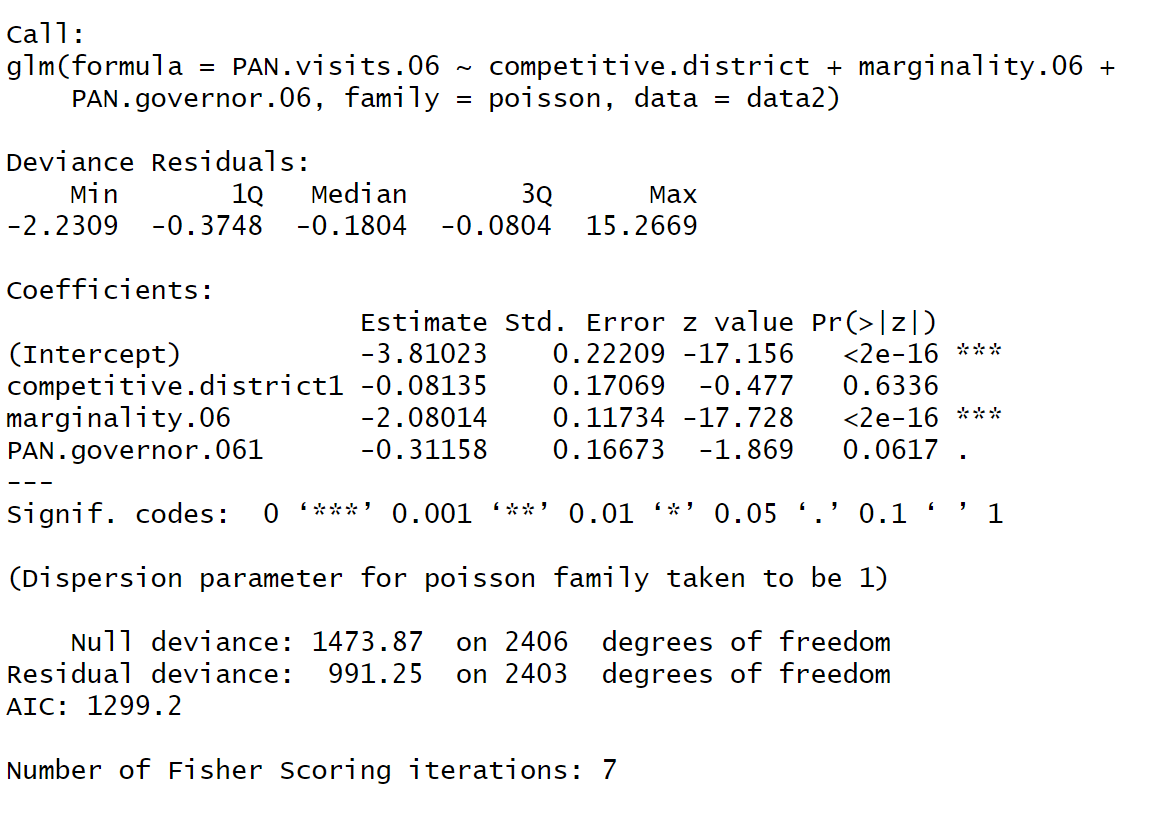
\includegraphics[width=.75\textwidth]{PoissonReg.png}
	 \end{figure} 

	The z-score test statistic (-0.477) indicates that there is not enough evidence to suggest that PAN presidential candidates visit swing districts more. This test score results in a P-value of 0.6336, which is above our critical threshold for rejecting the null hypothesis that being a competitive district has no effect on the number of visits.  

	\item [(b)]
	Interpret the \texttt{marginality.06} and \texttt{PAN.governor.06} coefficients.
	
	\vspace{.5cm}
	\textbf{Answer:}\\
	
	Exponentiating the coefficients generated by our model gives us the values in Figure 3. A one unit increase in the marginality of a municipality changes the average number of visits by a multiplicative factor of 0.125, holding the other variables \texttt{PAN.governor.06} and \texttt{competitive.district} constant. A one unit increase in \texttt{PAN.governor.06} (i.e. having a PAN governor) changes the average number of visits by a multiplicative factor of 0.732, holding the other variables \texttt{marginality.06} and \texttt{competitive.district} constant.
	
	\begin{figure}[H]\centering
		\caption{\footnotesize Exponentiated coefficients}
		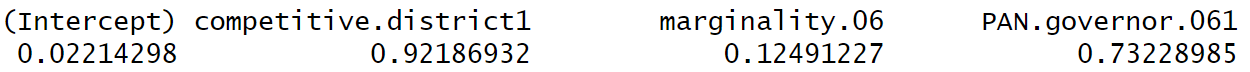
\includegraphics[width=.75\textwidth]{expCoeffs.png}
	\end{figure}
	
	\item [(c)]
	Provide the estimated mean number of visits from the winning PAN presidential candidate for a hypothetical district that was competitive (\texttt{competitive.district}=1), had an average poverty level (\texttt{marginality.06} = 0), and a PAN governor (\texttt{PAN.governor.06}=1).
	
	\vspace{.5cm}
	\textbf{Answer:}\\
	
	The estimated mean number of visits from the winning PAN presidential candidate for a hypothetical district that was competitive, had an average poverty level and a PAN governer was calculated using the below code:
	
	\vspace{.5cm}
	\lstinputlisting[language=R, firstline=99, lastline=102]{PS3_DanielMurray.R}  
	\lstinputlisting[language=R, firstline=107, lastline=108]{PS3_DanielMurray.R}  
	\vspace{.5cm}
	
	The value was calculated as 0.0149 visits.
	
\end{enumerate}

\end{document}
